%Layout
	\documentclass[a4paper, twocolumn, twoside, 12pt]{article}
	\setlength{\columnsep}{1cm}
	\setlength{\parskip}{6pt}
	%\usepackage{geometry}
	\usepackage[margin=1.5cm]{geometry}
	\usepackage{float}
	%\usepackage{multicol}
	\usepackage{tocloft}
	\renewcommand\cftsecafterpnum{\vskip-5pt}

%fonts
	\usepackage[T1]{fontenc}
	\usepackage[sfdefault]{roboto}
	\usepackage[T1]{fontenc}
	\usepackage[usenames, dvipsnames]{color}

%Code listings
	
	\usepackage{listings}
	\definecolor{code}{rgb}{0.95,0.95,0.95}
	\definecolor{codeframe}{rgb}{0.9,0.9,0.9}
	
	\lstset{
		frame=single,
		numbers=left,
		numbersep=10pt,
		tabsize=8,
		basicstyle=\footnotesize\ttfamily,
		rulecolor=\color{codeframe},
		backgroundcolor=\color{code}
		}

	%Python Specific
	\definecolor{pcomment}{RGB}{207,0,19}
	\definecolor{pkey}{RGB}{241,117,34 }
	\definecolor{pcode}{rgb}{0.95,0.95,1.0}
	\definecolor{pcodeframe}{rgb}{0.8,0.8,1.0}
	\definecolor{codenumber}{rgb}{0.5,0.5,0.5}
	
	\lstdefinestyle{python}{
		language=Python,
		rulecolor=\color{pcodeframe},
		backgroundcolor=\color{pcode},
		keywordstyle=\color{pkey},
		commentstyle=\color{pcomment},
		numberstyle=\tiny\color{codenumber},
		emphstyle=\color{purple},
		showstringspaces=false,
		tabsize=4,
		breaklines=true
		}
%Asides
	\usepackage{mdframed}
	\newenvironment{aside}
		{
		\begin{mdframed}[
			style=0,%
			leftline=false,
			rightline=false,
			innerbottommargin=2pt,
			innerleftmargin=12pt,
			innerrightmargin=0pt,
			linewidth=0.75pt,
			skipabove=6pt,
			skipbelow=6pt
			]
				\small
				\color{JungleGreen}
				\setlength{\parskip}{2pt}
				\vspace{2pt} %correct for parskip
		}
		{
		\end{mdframed}
		}

%Everything else
	\usepackage[utf8]{inputenc}
	\usepackage{graphicx}
	
%	-	-	-	-	-	-	-	-	-	-	-	-	-	-	-	-	-	-	-	-

\begin{document}

	\author{Manchester Raspberry Jam}
	\title{Workshop 8: Introduction to Sense HAT}
	\date{}

	\maketitle
	
	\setcounter{tocdepth}{1}
	\tableofcontents
	
%	-	PART 0
\setcounter{section}{-1}
	\section{Introduction}
		This is an introductory workshop on the features of the Sense HAT, and should be straightforward to complete, even if you haven't coded before.
		
		These booklets were created using {\fontfamily{rfdefault}\selectfont \LaTeX}, an advanced typesetting system for several sorts of books, reports and letters.
		
		To allow modification and redistribution of these booklets, they are distributed under the CC BY-SA 4.0 License.
	
	\subsection*{What you'll need}
		\begin{itemize}
			\item You'll need a Sense HAT board for your Raspberry Pi.
			\scriptsize\newline They can be purchased from \color{WildStrawberry}www.raspberrypi.org/products\color{black}, or anywhere that sells Raspberry Pis.
			\normalsize
			
			\item The Sense HAT API is pre-installed on new versions of Raspbian. (Jessie or later) 			
			\scriptsize\newline Make sure you download the latest version of it from \color{WildStrawberry}www.raspberrypi.org/downloads\color{black}
			\normalsize
			
			\item Download the files for this workshop from our Google Drive:
			\scriptsize\newline Go to \color{WildStrawberry}bit.ly/mcrraspjam\color{black}, then navigate to `Workshops $>$ 008: Sense HAT'.
			\normalsize
		\end{itemize}
	
	\subsection*{Programming with Python}
	
	We'll be coding in Python for this workshop, and we'll be using a program called IDLE to write our programs.
	
	It is an `IDE', containing a text editor to write our programs, as well as a Python `Shell' where we will run them.
	
	To start IDLE\label{IDLE}, go to the main menu from the Raspberry Pi's desktop, then click \mbox{`Programming $\rightarrow$ Python 3'}. IDLE will start after a couple of seconds.
	
	\subsection*{Code listings \& asides}
	
		When you need to make changes to your code, they'll be presented in boxes like the following:

		\lstinputlisting[style=python, firstline=1, lastline=6]{code/1_helloworld.py}
	
		You might not need to copy everything out, check the line numbers when in doubt.
	
		Occasionally, something will be explained in greater detail in asides, like the one below. You can read these as you wish.
	
		\begin{aside}
			Red lines beginning with the number signs (\#) are called \textbf{comments}.
			We use them to explain what each bit of code does, but they make no difference to how the program runs.
		\end{aside}
		
	\subsection*{Questions?}
	
		If you get stuck, or have suggestions for these booklets, you can send me an email at:
		\newline \color{WildStrawberry}jack@slightlyintelligent.com\color{Black}\label{email}
	
	\section{Weather station}
	
		The Sense HAT has a pair of environmental sensors, for temperature, atmospheric pressure, and relative humidity.
		We'll start with a simple script, which probes on of these sensors, and prints out the data as text on screen.
		
		\subsection*{weather.py}
		
		After opening IDLE, (see page \ref{IDLE}) click `File $\rightarrow$ Open...'.
		From the Home folder `pi', where you currently are, navigate to
		`workshops $\rightarrow$ 008\_senseHAT $\rightarrow$ morning'
		and open `weather.py'.
		
		\lstinputlisting[style=python, firstline=1, firstnumber=1, lastline=5]{code/weather.py}
		
			The first two lines of the script tell Python that this program will use the Sense HAT.
			The first line loads the `API', which allows us to program the Sense HAT in Python, and
			the second line runs some set-up procedures for our program.
			
			First, we'll add a basic print function, as a welcome message when running the program.
			
			\begin{aside}
				A \textbf{print function} will `print' text on-screen when the program is run.
				
				We put what we want to be printed inside the parentheses, text must be surrounded by quote marks.
			\end{aside}

		\lstinputlisting[style=python, firstline=6, firstnumber=6, lastline=8]{code/weather.py}
		
			You can try running your program now, by first saving, then going to \mbox{`Run $\rightarrow$ Run Module'}. The window should switch back to the one that first opened when we ran IDLE, and our text should turn up after a couple of seconds.
			
			The print statement is a simple start to our program, and we'll come back to them shortly, but now, let's try pulling data from the Sense HAT sensors:
			
		\lstinputlisting[style=python, firstline=9, firstnumber=9, lastline=11]{code/weather.py}
		
		We have used the Sense HAT function `hat.get\_temperature()' to get the temperature, in Celsius, from the sensor. It returns it as a number which we have stored in the variable `temperature'.
		
		\begin{aside}
			A \textbf{function} calls a piece of code that somebody else has written for us.
			
			A function can be identified by the pair of parentheses. print(), str() and round() are examples of functions.
			
			Some functions output, or `return' a value, they can also take inputs, called `parameters' which are placed within the parentheses.
		\end{aside}
		\begin{aside}
			When we store a number or other value in our program for later use, it is called a \textbf{variable}.
			
			We can give a variable any name we want, and we set a variable using: `variablename = value'
		\end{aside}
		
		We need to print out the number so we can see it when we run the program. We'll use another print function, but instead of text, surrounded by quotes, we'll use our variable `temperature' instead:
		
		\lstinputlisting[style=python, firstline=1, firstnumber=12, lastline=2]{code/weather_alt.py}
		
		str() is used to turn a number into a `string', the text representation of our number, as print() cannot print numbers without conversion.
		
		When you run this program, you'll see that the temperature is printed out with a high number of decimal points. (e.g. 29.852941513061523)
		This is a lot more than we need, so we can round the number down to less decimal places using another function round().
		
		round has two parameters, which we separate within the parentheses using commas, round(number, decimal places). In our code that looks like this:
		
		\lstinputlisting[style=python, firstline=5, firstnumber=11, lastline=8]{code/weather_alt.py}
		
		The program now outputs a temperature which is easy to read.
		One last thing we can do is add a label and unit when we print out the temperature.
		
		We can combine strings in the print function by adding them together.
		Instead of mathematical addition like numbers, Python will perform a `string concatenation'; basically, putting one string after another to make one big string.
		
		\lstinputlisting[style=python, firstline=14, firstnumber=14, lastline=14]{code/weather.py}
		
		Make sure each `string' of text is encapsulated in its own set of quotes, like above.
		
		\subsection*{Adding Humidity}
		
		Once we've gotten our heads around the temperature, we can use exactly the same steps for the humidity and pressure.
		
		\begin{aside}
			\textbf{Humidity} is a measure of the water vapour in the air, and is measured as a percentage \%.
			
			Water holds a lot of heat energy, which can increase temperatures. Humid air also slows down the rate at which we can sweat, which can make hot temperatures even more unbearable!\textsuperscript{\cite{humidity}}
		\end{aside}
		
		Instead of using the get\_temperature() function, we just need to use the `get\_humidity()' function instead. Everything else is the same, so we can copy and paste our code, and change the variable names and text labels.
		
		\lstinputlisting[style=python, firstline=15, firstnumber=15, lastline=20]{code/weather.py}

		\subsection*{Adding Atmospheric Pressure}		
		Finally, we can do atmospheric pressure. This time the function is called get\_pressure(). Have a go at this implementing this last measurement yourself.
		\begin{aside}
			\textbf{Atmospheric pressure} is caused by the weight of air from the atmosphere, and is measured in millibars.
			
			As altitude increases, the amount of air in the atmosphere starts to decrease (referred to as thin air), resulting in a lower pressure. Pressure is also affected by temperature, with local differences affecting winds. Low pressure is associated with high cloud cover and precipitation.
			\textsuperscript{\cite{pressure}}
		\end{aside}
		
	\section{G-Force}
	
		As well as the environmental sensors, the Sense HAT has a set of inertial momentum unit (motion and orientation) sensors. These are used primarily for determining the orientation of your Pi, which we'll use this afternoon.
		
		For now, we'll use the raw accelerometer data to measure the 'G-force' under various scenarios.
		
		\begin{aside}
			\textbf{G-forces} are a measure of acceleration acting on an object, relative to 1G, the acceleration due to the force of gravity. A still object like our Pi is experiencing 1G downwards.
			
			Here are a few interesting examples of different situational G-forces:\textsuperscript{\cite{gforce}}
			\color{Black}
			\begin{tabular}{|c|c|}
				\hline \textbf{Example} & \textbf{G-force} \\ 
				\hline Gravity on the Moon & 0.165 \\ 
				\hline Gravity on the Earth & 1 \\ 
				\hline Space Shuttle launch & 3 \\ 
				\hline Top Fuel dragster & 4.2 \\ 
				\hline High-G roller coaster & 3.5 - 6 \\ 
				\hline Jet fighter manoeuvre & 9 - 12 \\ 
				\hline Human on Rocket sled test & 46.2 \\ 
				\hline Bullet in gun barrel & 60,000 \\ 
				\hline Proton in LHC & 190,000,000 \\ 
				\hline 
			\end{tabular}
		\end{aside}
		
		\subsubsection*{gforce.py}
		
			Click \mbox{`File $\rightarrow$ Open...'}.
			From the home folder, go to \mbox{`workshops $\rightarrow$ 008\_senseHAT $\rightarrow$ morning'} and open `gforce.py'.
		
			Like before, we'll be calling an API function to fetch the sensor data. get\_accelerometer\_raw() returns a vector, with x, y and z axis `components'.
		
			\lstinputlisting[style=python, firstline=1, firstnumber=1, lastline=6]{code/gforce_alt.py}
		
			We've seen vectors before, used in Minecraft: Pi Edition's APIs, but this time the function has returned the three components within a `dictionary' data structure, rather than a list, as used previously. We'll need to know how to access the individual components to round them.
		
			\begin{aside}
				\textbf{A dictionary} is quite similar to a list in Python. A list is a group of variables, each referenced by a number. A vector (13, 24, 17) in a list would look like:
				
				\color{Black}
				\begin{tabular}{|c|c|}
					\hline Index & Value \\ 
					\hline 0 & 13 \\ 
					\hline 1 & 24 \\ 
					\hline 2 & 17 \\ 
					\hline 
				\end{tabular} 
				\color{JungleGreen}
				
				The $y$ component would be accessed with: \mbox{Vector[1]}
				
				A Dictionary uses text indices instead of numerical ones. This may be more intuitive to you, but it also makes dictionaries great for data with no inherent ordering. If you want to use a dictionary in your own programs, you can define one like so:
				\mbox{dictionary = \{'x': 13, 'y': 24, 'z': 17\}}
				
				Which means a dictionary for that vector would look like:

				\color{Black}
				\begin{tabular}{|c|c|}
					\hline Index & Value \\ 
					\hline 'x' & 13 \\ 
					\hline 'y' & 24 \\ 
					\hline 'z' & 17 \\ 
					\hline 
				\end{tabular}
				\color{JungleGreen}
				
				The $y$ component would be accessed with: \mbox{Vector['y']}	
			\end{aside}
			
			We can now access each component and round it, returning it back to the dictionary
			
			\lstinputlisting[style=python, firstline=7, firstnumber=7, lastline=10]{code/gforce_alt.py}
			
			We now have rounded all of the 3 G-Force Values, and we can print them.
			Luckily Python will neatly print out all of the components of a data structure like a dictionary, we can just to pass it to the print function:
			\lstinputlisting[style=python, firstline=11, firstnumber=11, lastline=11]{code/gforce_alt.py}
			
			You can now run your program. Make sure your Raspberry Pi is flat on the desk, can you figure out which axis is the up/down axis, based on the numbers?
			
			One final modification to our program. It'd be nice to measure G's changing as we move the Raspberry Pi about, so we'll encapsulate our program in an infinite loop, like so:
			
			\lstinputlisting[style=python, firstline=5, firstnumber=5]{code/gforce.py}
			
			Rerun the program, and experiment with the different G-forces you can create.
			
			By rotating your pi to stand on different sizes, you can change the axis and polarity of gravity. By shaking your pi you can cause brief forces in directions
			other than that of gravity. If you were to drop your Pi on a hard surface, you might see G spikes in the 10's or 100's, consistent with crash forces.
	
	\section{G-Force Demonstration}
	
		We'll take a look at a few applications for the G-force sensor now. There's no coding for this section, we'll just be looking at some interesting examples.
		
		With a small adjustment to our code, we can output to a text file, instead of to the Python shell. I chose to output the captured telemetry in CSV format.
		
		\begin{aside}
		\textbf{CSV} formatted data is a simple text format, where data is separated into rows, separated by columns. For example, the following CSV data:
		\color{Black}
		\newline time, x, y, z\newline
		0.0, 0.97, 0.03, 0.01\newline
		0.1, 0.98, 0.02, 0.01
		\color{JungleGreen}
		
		is equivalent to a spreadsheet table:
		\color{Black}
		\begin{tabular}{|c|c|c|c|}
			\hline time & x & y & z \\ 
			\hline 0.0 & 0.97 & 0.03 & 0.01 \\ 
			\hline 0.1 & 0.98 & 0.02 & 0.01 \\ 
			\hline 
		\end{tabular}
		\end{aside}

		Many pieces of software will accept CSV as data input, we'll look at two pieces of software, \mbox{Wolfram Mathematica} and \mbox{Libreoffice Calc}. (a spreadsheet software)
		
		\iffalse
		
		\subsubsection*{Elevator G-force}
		
		Anything which accelerates or decelerates will produce a measurable G-force. One everyday example is an elevator. As the elevator begins its journey, it accelerates upwards, producing G-forces, and as it reaches the top of its journey, we expect the G-forces to decrease.
		
		To test this, I powered my Pi with a USB battery pack, and ran the G-force CSV program. I then imported the data into \mbox{Wolfram Mathematica}.
		
		\textit{I won't detail the process in this workshop, but the commands you need are Import[] and \mbox{ListLinePlot[]}}
		
		\begin{center}
			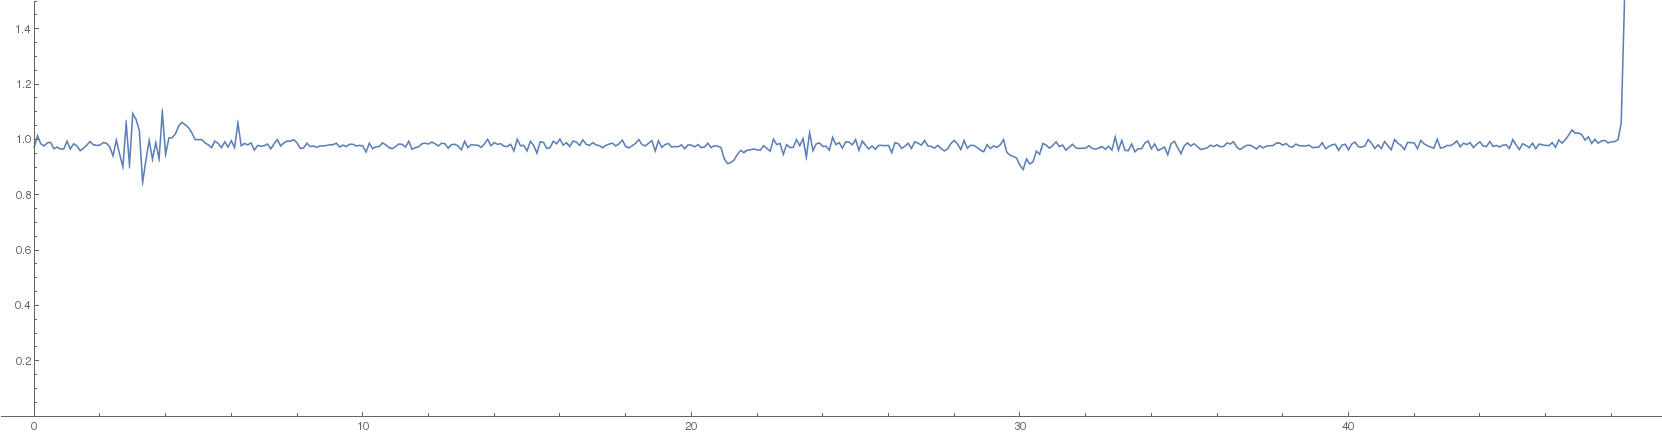
\includegraphics[width=1\linewidth]{img/Results_Mathematica}
		\end{center}
		
		The forces involved with the elevators operation are very small. For context, the spikes at the start of the graph are me taking a step towards the elevator button.
		
		At the end of this spike, you see a single wide spike, lasting about 1 second; this is the elevator accelerating upwards. Acceleration then returns to zero as the elevator reaches its travelling speed. the next spike is in the opposite direction, as the elevator reaches the top floor of the building. There are two additional spikes, for the return journey.
		
		We can determine a few things from this data. The acceleration of elevator seems to be about $0.1G$ in both directions, or just under $1ms^{-2}$. In addition, the duration of the journey is from the start of the acceleration spike to the end of the deceleration spike, meaning each of the two journeys took about 27 seconds.
		
		\fi

		\subsubsection*{Dropping the Pi}
		
		Elevator forces are bit pedestrian, far more exciting is the prospect of Zero-G. Astronauts onboard the ISS experience `microgravity' in orbit around the earth, but we can also experience brief moments of zero G-force on earth.
		
		\begin{aside}
			Objects in \textbf{free-fall} are accelerating with gravity, and feel no resisting forces from the ground; They measure 0G.
			
			We can experience zero-G in earth, essentially by strapping ourselves to "falling" objects, such as the `Vomit comet', a plane manoeuvre made infamous by NASA, in their astronaut training.
		\end{aside}
		
		It stands to reason that by dropping our Pi, whilst recording G-force data, we could measure a moment of zero-G. In the hope of preventing you from destroying your Pi, we decided to test it ourselves.
		
		We dropped the Pi from a balcony, about a storey high, and caught it from below. We imported the resulting CSV file into \mbox{Libreoffice Calc}, and created a graph.
		
		\begin{center}
			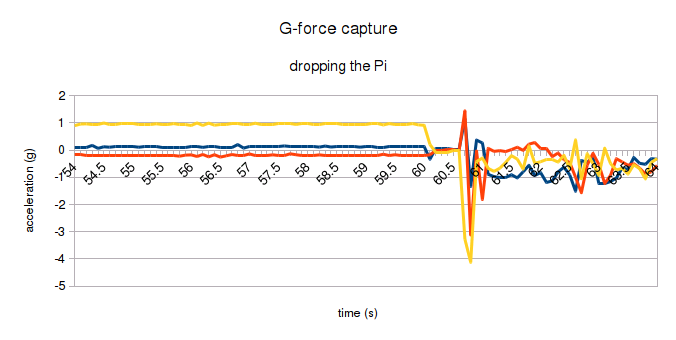
\includegraphics[width=1\linewidth]{img/graph_whole}
		\end{center}
		
		You can probably see the drop point on the graph. When held on the balcony, the Z-axis shows a steady 1G under gravity, until it is dropped, where it drops to zero. The large spike is the force exerted as I catch the Pi. Let's look closer at that section:

		\begin{center}
			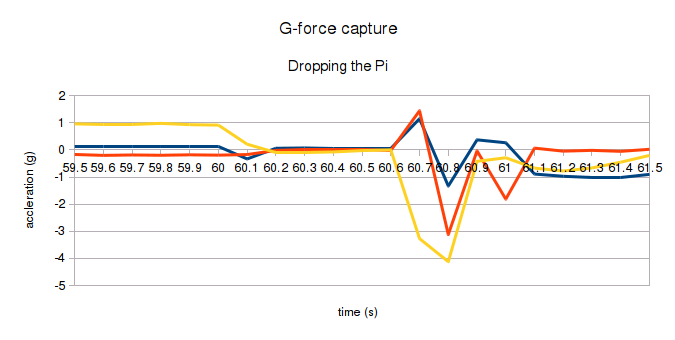
\includegraphics[width=1\linewidth]{img/graph_detail}
		\end{center}
		
		Our recorded data looks perfect, we can see consistent 0G in free-fall, just as we predicted. What's more, by getting the duration of free-fall (which I make to be 0.5s), we can work out some more details of our drop.
		
		There are a set of mathematical formulas for Constant acceleration, such as under gravity, which you may use in A-level Physics. Don't worry though, they're really simple when calculating gravity! One of those is as follows:
		
		$v = u + at$
		
		We want to find `v', the speed at the end of the drop. `u' is the speed at the start of the drop, which is 0. `a' is acceleration due to gravity, which is always $9.81m/s^{2}$. `t' is the time in free-fall, which we measured as $0.5s$.
		
		$v = 0 + 9.81 \times 0.5$
		
		$= 9.81 \times 0.5$
		
		$v = 4.9 m/s$
		
		Which means that the Raspberry Pi was caught at over 10 miles per hour!
		
	\section{Motion controlled Snake}
	
		In workshop 7, we created a simple version of the video game Snake, on the unicorn HAT board.
		
		In this workshop, we'll be modifying the game to make the snake move based on how we tilt the Raspberry Pi, rather than using keyboard controls.

	\subsection*{snake.py}
	
		Click `File $\rightarrow$ Open...'.
		Go to `workshops $\rightarrow$ 008\_senseHAT $\rightarrow$ afternoon' and open `snake.py'.
		
		\textit{Note: because the snake game was originally written for the Unicorn HAT, all of the hat functions are accessed by \textbf{UH.<command>}, not hat.<command> as in the earlier programs.}
		
		If you attended our previous workshop, this is the same code you completed previously.
		
		As we are working with an already complete and playable version of the game, I have separated the control inputs into a separate function, called `get\_input'.

		\lstinputlisting[style=python, firstline=16, firstnumber=16, lastline=30]{code/snake_old.py}
			
		This bit of code checks each keyboard key, and if pressed, will change the direction the snake (player) is travelling. Direction is a number, where 0 signifies up, 1 is right, 2 is down, and 3 is left.
		
		Our version of the code will follow the same steps, but rather than using keyboard input, we will use
		
		Our function will follow the same steps, except rather than 
		
	\subsection*{Rewriting get\_input}
		
		First we need to determine to get the G-forces from the Sense HAT. We will store it as a variable, as we did earlier
		
		\lstinputlisting[style=python, firstline=16, firstnumber=16, lastline=19]{code/snake.py}
		
		Before we can return the correct direction, we need to know which direction we need to move in based on the direction of tilt. Rerun your looping G-force program, and record the G measurements for each of the 4 directions.
		
		\textit{\scriptsize Remember that the HDMI port is at the "bottom" of game board, and the snake should move ``downhill'', so to move up, you will tilt the top of the Pi downwards.}
		
		The directions I determined are below:
		
		\begin{tabular}{|c|c|}
			\hline Axis & Direction \\ 
			\hline X+ & 1 \\ 
			\hline X- & 3 \\ 
			\hline Y+ & 2 \\ 
			\hline Y- & 0 \\ 
			\hline 
		\end{tabular}
		
		Then, it is simply a matter of rewriting the old function, but with appropriate x/y values for each direction:
		
		\lstinputlisting[style=python, firstline=21, firstnumber=21, lastline=28]{code/snake_mid.py}
		
		I have chosen values greater than 0.3, as we want a control `deadzone', so the direction does not change erratically when we try to hold our Raspberry Pi flat.
		
		We are more or less finished, and your game should now be playable.
		
		A final modification I would consider making is to disallow movement changes when holding the Pi diagonally, as currently certain directions are chosen before others which may also be satisfied. I'll leave for you, with a hint below.
		
		\scriptsize{
			\textbf{Hint:} change the if statement as above to an elif, and add a first if before. Use the boolean \textbf{and} and \textbf{or} operators to combine comparisons for your condition. Solution at github.com/McrRaspJam
		

\begin{thebibliography}{9}
	\scriptsize{
	\bibitem{humidity}
	https://en.wikipedia.org/wiki/Humidity
	
	\bibitem{pressure}
	https://en.wikipedia.org/wiki/Atmospheric\_pressure
	
	\bibitem{gforce} 
	https://en.wikipedia.org/wiki/Orders\_of\_magnitude\_(acceleration)
	}
\end{thebibliography}

\end{document}